\section{Ejericio 7}

\subsection{Scheduler, debugger y etcs}

En este punto, se nos pide inicializar las estructuras necesarias para el scheduler. Para esto, tenemos la función \texttt{sched\_inicializar} que setea como jugador actual al jugador A, y como pirata actual de ambos jugadores al 0.

Las funciones \texttt{sched\_tick}, \texttt{game\_proximo\_pirata} y \texttt{sched\_proxima\_a\_ejecutar}, también implementadas en este punto, fueron detalladas anteriormente, así como también el desarrollo de la rutina de la interrupción 0x46 para que atienda los servicios de mover, cavar y dar la posición de un pirata.

Por último, implementamos el mecanismo de debugging pedido en el enunciado, en el que al presionar la tecla Y se accede al modo debug, y en cuanto se produzca una excepción se mostrará en pantalla el estado del procesador tal como se muestra en la figura.

\begin{figure}[ht]
\centering
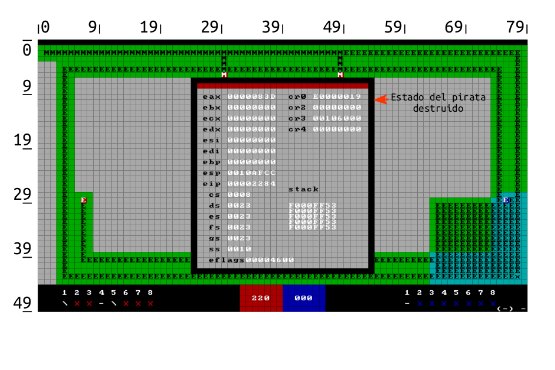
\includegraphics[width=90mm]{ej_7/img_ej_7.png}
\end{figure}

Al presionar nuevamente la tecla Y, se borra la información presentada en pantalla y se desaloja la tarea que produjo la excepción y se salta a la tarea Idle hasta que se decida en el próximo ciclo de reloj cual es la próxima tarea a ser ejecutada.
Para realizar esto, en la macro realizada para las excepciones de la 1 a la 19, se chequea si nos encontramos en el modo debug. De no ser así, retornamos sin hacer nada. Si estábamos en modo debug, se salva el estado actual de la pantalla con \texttt{screen\_pantalla\_debug} y se queda ciclando hasta que se detecte que se presionó nuevamente la tecla Y. Cuando esto suceda, se llama a \texttt{load\_screen} que restablece la pantalla previa y a continuación se llama a \texttt{game\_pirata\_exploto}, que setea al pirata actual como muerto, y resta uno a la cantidad de piratas del jugador correspondiente. A su vez, setea el bit de presente del descriptor en GDT del pirata muerto como 0 y actualiza el reloj del pirata en la pantalla con \texttt{screen\_actualizar\_reloj\_pirata}. 
Finalmente se setea como próximo selector al de la tarea Idle y se realiza un jmp far a esta.
El flag de modo debug se setea en 0 o 1 (de acuerdo al valor previo del flag) en \texttt{game\_atender\_teclado} cuando se detecta que la tecla presionada fue Y.
La función \texttt{screen\_pantalla\_debug} salva el estado inicial de la pantalla con \texttt{save\_screen} y printea en pantalla la pantalla de debug según se muestra en la ilustración, con los datos correspondientes para la tarea que lanzó la excepción.
Como cuando se lanza una excepción de una tarea nivel que está corriendo en nivel 3 se cambia el nivel de privilegio y este pasa a ser 0, se guardan en el stack varios parámetros que usaremos para mostrar en pantalla de debug, ya que estos argumentos obtenidos de la pila son usados como sus parámetros. Además, como utilizamos la instrucción pushad antes de llamar a la función, guardamos en la pila todos los registros de propósito general. 


